\documentclass[a4paper,11pt]{ltjsarticle}

% --- パッケージの読み込み ---
\usepackage{amsmath, amssymb, amsthm, mathrsfs}
\usepackage{luatexja}
\usepackage{tikz}
\usetikzlibrary{cd, shapes, backgrounds, positioning, calc, arrows.meta, fit, patterns, trees}
\usepackage{hyperref}
\usepackage{xcolor}
\usepackage{listings}
\usepackage{tcolorbox}
\usepackage{booktabs}
\usepackage{multicol}

% --- ハイパーリンク設定 ---
\hypersetup{
    colorlinks=true,
    linkcolor=blue!70!black,
    citecolor=blue!70!black,
    urlcolor=blue!70!black
}

% --- 定理環境の定義 ---
\theoremstyle{definition}
\newtheorem{definition}{定義}[section]
\newtheorem{theorem}[definition]{定理}
\newtheorem{lemma}[definition]{補題}
\newtheorem{example}[definition]{例}
\newtheorem{remark}[definition]{注釈}

% --- マクロ定義 ---
\newcommand{\N}{\mathbb{N}}
\newcommand{\Z}{\mathbb{Z}}
\newcommand{\Q}{\mathbb{Q}}
\newcommand{\R}{\mathbb{R}}
\newcommand{\C}{\mathbb{C}}
\newcommand{\Tower}{\mathcal{T}}
\newcommand{\Layer}[1]{\mathrm{Layer}_{#1}}
\newcommand{\MinLayer}{\mathrm{minLayer}}

% --- タイトル情報 ---
\title{\textbf{構造塔の萌芽と展開：ブルバキ流形式化の旅路} \\ \large --- Lean 4による現代数学の統一的記述 ---}
\author{
    Lean Code Generation: \textbf{CODEX (OpenAI)} \\
    TeX Explanation \& Typesetting: \textbf{Gemini (Google)}
}
\date{\today}

\begin{document}

\maketitle

\begin{abstract}
本稿では、一連のLean 4ファイルに基づき、ブルバキ『数学原論』の精神を受け継ぐ形式化の試みについて解説する。特に、順序集合上の単調な集合族を抽象化した「構造塔 (Structure Tower)」という概念に着目し、それが集合論の基礎から始まり、代数（イデアル、ガロア接続）、位相（閉包、フィルター）、そして解析学やネーター環論へとどのように応用・発展していくかを体系的に記述する。
\end{abstract}

\tableofcontents
\newpage

% =========================================================================
% Section 1: Bourbaki_Lean_Guide
% =========================================================================
\section{構造塔の萌芽：Bourbaki\_Lean\_Guide}
\label{sec:bourbaki_guide}
\textit{Based on: \texttt{Bourbaki\_Lean\_Guide.md}}

全ての始まりは、数学的対象を「階層構造」として捉える視点にある。

\subsection{ポセットと上限の一意性}
まず、半順序集合 (Poset) における上限 (Least Upper Bound) の一意性が確認される。これは、構造が一意に定まるための基礎である。

\subsection{StructureTower の定義}
本プロジェクトの中核をなす `StructureTower` は、順序集合 $\iota$ で添字付けられた、単調増加する集合族として定義される。

\begin{definition}[Structure Tower]
型 $\alpha$ 上の構造塔とは、前順序集合 $\iota$ と写像 $\mathrm{level}: \iota \to \mathrm{Set}\ \alpha$ の組であり、以下を満たす。
\[ i \le j \implies \mathrm{level}(i) \subseteq \mathrm{level}(j) \]
\end{definition}

この単純な定義が、後の章で驚くべき汎用性を発揮する。

\begin{figure}[h]
\centering
\begin{tikzpicture}
    % Base set
    \draw[fill=gray!5] (0,0) ellipse (3cm and 2cm);
    \node at (0, -2.5) {全体空間 $\alpha$};

    % Levels
    \draw[fill=blue!10, draw=blue] (0,-1) circle (0.5cm);
    \node[blue] at (0, -1) {$L_0$};

    \draw[fill=blue!20, draw=blue, fill opacity=0.5] (0,-0.5) ellipse (1.5cm and 1cm);
    \node[blue] at (0, 0) {$L_1$};

    \draw[fill=blue!30, draw=blue, fill opacity=0.3] (0,0) ellipse (2.5cm and 1.8cm);
    \node[blue] at (0, 1.5) {$L_2$};

    % Inclusion arrow
    \draw[->, thick] (0.8, -1) -- (1.8, -0.5);
    \node at (2.5, -1) {単調性};
\end{tikzpicture}
\caption{構造塔のイメージ。順序に従って領域（層）が拡大していく。}
\end{figure}

\subsection{具体例：自然数の初期区間}
自然数 $\N$ 自身も構造塔と見なせる。
\[ \mathrm{level}(n) = \{k \in \N \mid k \le n\} \]
この塔の和集合は $\N$ 全体となる。これは「全ての自然数はある有限の深さを持つ」ことを意味する。

% =========================================================================
% Section 2: P1 - 基礎的演習
% =========================================================================
\section{基礎構造の確認：P1}
\label{sec:p1}
\textit{Based on: \texttt{P1.md}}

構造塔を構築するための「レンガ」となる基礎的な数学的対象（順序、群、位相）の性質を確認する。

\begin{itemize}
    \item **順序**: 推移律、上限の性質。
    \item **束**: 分配律、部分分配律。
    \item **群**: 準同型の像 `imageSubgroup` が部分群をなすこと。これは後の「構造を保存する射」の基礎となる。
    \item **位相**: コンパクト集合の閉性、ハウスドルフ空間での分離公理。
\end{itemize}

これらは個別の定理に見えるが、ブルバキ流の「母構造」の視点では、これらが組み合わさってより複雑な構造（トポロジカルグループなど）が形成される。

% =========================================================================
% Section 3: P1\_Extended - 閉包とガロア接続
% =========================================================================
\section{閉包作用素と構造塔：P1\_Extended}
\label{sec:p1_extended}
\textit{Based on: \texttt{P1\_Extended.md}}

ここで、構造塔の生成原理の一つである「閉包作用素」と「ガロア接続」が登場する。

\subsection{ガロア接続 (Galois Connection)}
二つの順序集合間の随伴関手対 $(l, u)$ はガロア接続と呼ばれる。
\[ l(a) \le b \iff a \le u(b) \]
これは、代数幾何学における「イデアル」と「代数的集合」の対応など、数学の至る所に現れる構造である。

\subsection{Bourbaki 閉包作用素}
閉包作用素 $c: \alpha \to \alpha$ は、単調性、広義単調性 ($x \le c(x)$)、巾等性 ($c(c(x)) = c(x)$) を満たす。
これを用いると、自然な構造塔が定義できる。
\[ \mathrm{level}(x) = \{y \in \alpha \mid y \le c(x)\} \]
これは「$x$ によって生成される（閉包に含まれる）要素の集合」を層とする塔である。

\begin{figure}[h]
\centering
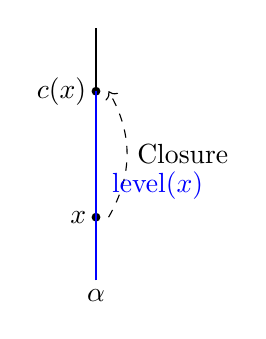
\begin{tikzpicture}[scale=0.8]
    % Poset Alpha
    \draw (0,0) -- (0,4);
    \node[below] at (0,0) {$\alpha$};
    \node[left] at (0,1) {$x$};
    \fill (0,1) circle (2pt);

    % Closure
    \node[left] at (0,3) {$c(x)$};
    \fill (0,3) circle (2pt);
    \draw[->, dashed] (0.2, 1) to[bend right] (0.2, 3);
    \node[right] at (0.5, 2) {Closure};

    % Tower level
    \draw[thick, blue] (0,0) -- (0,3);
    \node[blue, right] at (0.1, 1.5) {$\mathrm{level}(x)$};
\end{tikzpicture}
\caption{閉包作用素による構造塔。$c(x)$ 以下の全ての要素が層を形成する。}
\end{figure}

その他、連結性やウリゾーンの補題など、位相空間論における重要な構成も扱われている。

% =========================================================================
% Section 4: P1\_Extended\_Next - 代数とフィルター
% =========================================================================
\section{代数系とフィルターへの応用：P1\_Extended\_Next}
\label{sec:p1_extended_next}
\textit{Based on: \texttt{P1\_Extended\_Next.md}}

構造塔の概念を、可換環論やフィルター理論へ具体的に適用する。

\subsection{イデアルの塔 (Ideal Tower)}
環 $R$ のイデアル全体を `StructureTower` と見なす。
\[ \mathrm{level}(I) = I \quad (\text{集合としてのイデアル}) \]
単調性はイデアルの包含関係に対応する。全ての元 $x \in R$ は単項イデアル $(x)$ に含まれるため、この塔は全体 $R$ を被覆する。

\subsection{フィルターの塔 (Filter Tower)}
フィルター $F$ に対し、集合 $A$ をインデックスとする塔を定義する。
\[ \mathrm{level}(A) = \{x \in X \mid A \in F \land x \in A\} \]
これは「フィルター $F$ に属する集合 $A$ の要素」を層とするもので、収束の概念を階層化する視点を提供する。

\subsection{可測構造 (Sigma Algebra)}
可測空間における $\sigma$-代数もまた、集合族として構造塔の枠組みで捉えられる。`measurableTower` は、可測集合によって空間を階層化する。

% =========================================================================
% Section 5: P2\_Advanced\_Analysis - 解析学
% =========================================================================
\section{解析学における階層構造：P2\_Advanced\_Analysis}
\label{sec:p2}
\textit{Based on: \texttt{P2\_Advanced\_Analysis.md}}

ここでは、構造塔の概念が解析学（測度論・関数解析）においてどのように現れるかを確認する。

\begin{itemize}
    \item **可測集合の増大列**: 可算和の可測性は、$\sigma$-代数の塔における極限操作と見なせる。
    \item **単調収束定理**: 関数列 $f_n$ が単調増加するとき、積分の値も単調増加し、極限と交換可能になる。これは関数の構造塔における保存則である。
    \item **バナッハ・シュタインハウスの定理**: 作用素の族が一様有界であるための条件。これも作用素ノルムによる階層構造の性質である。
\end{itemize}

% =========================================================================
% Section 6: P3_Solved_NoetherianAndGalois - ネーター性とガロア
% =========================================================================
\section{ネーター環とガロア接続の深化：P3}
\label{sec:p3}
\textit{Based on: \texttt{P3\_Solved\_NoetherianAndGalois.md}}

最後に、構造塔の理論が現代的な代数学の核心部分（ネーター性とガロア理論）にどう接続されるかを見る。

\subsection{ネーター環と停止する塔}
環 $R$ がネーター的であるとは、イデアルの昇鎖 $I_0 \subseteq I_1 \subseteq \dots$ が停留することを意味する。
これを構造塔で表現すると、「イデアル鎖によって定義されるフィルトレーション塔 `filtrationTower` が、ある有限の高さで安定化する」ということになる。

\begin{theorem}[ネーター塔の安定化]
ネーター環上のイデアル昇鎖から作られる構造塔において、その和集合はある有限段階の層（イデアル）と一致する。
\[ \bigcup_{n} \mathrm{level}(n) = \mathrm{level}(N) \quad (\exists N) \]
\end{theorem}

\begin{figure}[h]
\centering
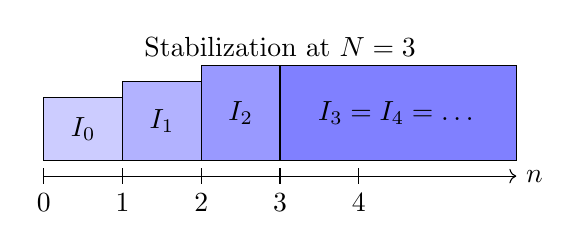
\begin{tikzpicture}
    \draw[->] (0,0) -- (6,0) node[right] {$n$};
    \foreach \x in {0,1,2,3,4} {
        \draw (\x,0.1) -- (\x,-0.1) node[below] {\x};
    }
    
    \draw[fill=blue!20] (0,0.2) rectangle (1,1); \node at (0.5,0.6) {$I_0$};
    \draw[fill=blue!30] (1,0.2) rectangle (2,1.2); \node at (1.5,0.7) {$I_1$};
    \draw[fill=blue!40] (2,0.2) rectangle (3,1.4); \node at (2.5,0.8) {$I_2$};
    \draw[fill=blue!50] (3,0.2) rectangle (6,1.4); \node at (4.5,0.8) {$I_3 = I_4 = \dots$};
    
    \node[above] at (3,1.4) {Stabilization at $N=3$};
\end{tikzpicture}
\caption{ネーター環におけるイデアルの昇鎖の停止。構造塔が「天井」にぶつかる様子。}
\end{figure}

\subsection{ガロア接続と完備束}
P1\_Extended で導入されたガロア接続を、完備束上で再考する。ガロア閉包 $c(x) = u(l(x))$ の不動点は完備束をなす。
これにより、「ガロア接続から誘導される構造塔 `galoisTower`」が定義され、その層構造（閉包による階層）が明確になる。

\section{結論}

これら一連のファイルは、**Structure Tower（構造塔）**という一つの抽象的概念が、集合論の基礎から始まり、位相、測度、そしてネーター環やガロア理論といった高度な代数構造に至るまで、数学の広範な領域を貫く「背骨」となり得ることを示している。
これは、ブルバキが目指した「数学の統一的記述」を、現代の定理証明支援系 Lean 上で具現化する試みと言えるだろう。

\end{document}